\section{Results}\label{sec:results}


In this section, we detail the findings of our study.  We remind the reader that our main goal with this study is to
better understand the strengths and limitations of the \mas for malware detection using the state-of-the-art
test case generation tool (DroidBot). We explore
the results of our research in two datasets: the \sds (102 pairs of apps) and the
\cds (\apps pairs of apps).


\subsection{Exploratory Data Analysis of Accuracy}


{\bf \sds.}
After running the dynamic analysis via DroidBot, our infrastructure produces
a dataset with the sensitive methods that both app versions call during their execution. We consider that a test
generation tool, in our case, DroidBot, builds a sandbox that labels a repackaged version
of an app as a malware if there is at least one call to a sensitive method that (a) was observed
while executing the repackaged version of the app and that (b) was not observed while
executing the original version of the same app. 
If the set of sensitive methods that only the repackaged version of an app calls is empty,
we conclude that the sandbox does not label the repackaged version the app as a malware. We triangulate
this information with the outputs of \vt, which might lead to one of the following
situations:

\begin{itemize}
\item {\bf True Positive}. The \mas labels a repackaged version as a malware and, according to
  \vt, at least two \ses label the asset as a malware.
  
\item {\bf True Negative}. The \mas does not label a repackaged version as a malware and,
  according to \vt, at most one \se labels the asset as a malware. 

\item {\bf False Positive}. The \mas labels a repackaged version as a malware and, according to
  \vt, at most one \se labels the asset as a malware.

\item {\bf False Negative}. The \mas does not label a repackaged version as a malware, and
  according to \vt, at least two \ses label the asset as a malware.
\end{itemize}



Considering the \sds (102 apps), the \mas for malware detection 
classifies a total of 69 repackaged versions as malware (67.64\%).
This result is close to what Bao et al. report. That is, in their
original paper,  the \mas approach using DroidBot classifies 66.66\% of the
repackaged version of the apps as malware~\cite{DBLP:conf/wcre/BaoLL18}.
This result confirms that we were able to reproduce
the findings of the original study using our
infrastructure. 

\tb{1}{We were able to reproduce the results of
  existing research using our infrastructure,
  achieving a malware classification in the
  \sds close to what has been reported in
  previous studies.}

In the previous studies~\cite{DBLP:conf/wcre/BaoLL18,DBLP:journals/jss/CostaMMSSBNR22},
the authors assume that all repackaged versions contain a
malicious behavior. For this reason, the authors do not
explore accuracy metrics such as Precision, Recall, and
F-measure ($F_1$). As we mentioned, in this paper we take advantage
of \vt to label our dataset and build a ground truth: we only
consider a repackaged version of an app a malware if the results
of our \vt query report that at least two
\ses identify a malicious behavior in the asset.
The first row of Table~\ref{tab:accuracy} shows that the
vanilla \mas achieves an accuracy of 0.89. 

\begin{table*}[htb]
  \caption{Accuracy of the \mas in both datasets.}
\centering{
  \begin{tabular}{llrrrrrr} \toprule
    Approach       & Dataset & TP   & FP  & FN  & Precision & Recall & $F_1$ \\ \midrule
    Vanilla \mas   & \sds    & 62   & 7   & 7   & 0.89      & 0.89   & 0.89  \\
    \mas + Traces  & \sds    & 67   & 18  & 2   & 0.78      & 0.97   & 0.87  \\
    Vanilla \mas   & \cds    & 173  & 173 & 286 & 0.5       & 0.37   & 0.42  \\
    \mas + Traces  & \cds    & 214  & 326 & 245 & 0.39      & 0.46   & 0.42  \\ \bottomrule
  \end{tabular}
  }
  \label{tab:accuracy}
\end{table*}

We also investigate if one could improve the performance of
the \mas using a more elaborated comparison approach.
That is, instead of only comparing the sets of calls to sensitive APIs,
here we also compare the traces from entry points to such a calls. If there is
at least one trace that appears only during the execution of the
test cases in the repackaged version of the app, we
label that version as a malware.

As we already discussed in this section, the vanilla \mas fails
to detect seven malware on the \sds (FN column, first row of Table~\ref{tab:accuracy}),
using DroidBot as a test case generator tool. Introducing trace analysis reduces the
number of false negatives to two, with the side effect of increasing the
number of false positives from 7 to 18 (see the second row of Table~\ref{tab:accuracy}).
In general, the accuracy ($F_1$) of the \mas using trace analysis drops from 0.89 to 0.67.


\tb{2}{Although the use of Trace Analysis reduces the number of
  false negatives (in comparison with the vanilla \mas), it slightly decreases the
  overall accuracy ($F_1$) of the \mas to detect malware,
  from 0.89\% to 0.87\% in the \sds.} 



{\bf \cds.} Surprisingly, when applied to our complete dataset (\apps apps), the \mas
labels a total of 346 repackaged apps as malware (28.76\% of the total number of repackaged
apps)---for which the repackaged version calls at least one additional sensitive API.
Our analysis also reveals a {\bf negative result} related to the accuracy of the approach: here,
the accuracy is much lower in comparison to what we reported for the
\sds (see the third row of Table~\ref{tab:accuracy}), dropping from 0.89 to 0.42 (a reduction of 47.19\% in terms of $F_1$).
This result indicates that, when considering a more representative dataset, the accuracy of the \mas using
DroidBot drops significantly. 


\tb{3}{
  The \mas for malware detection
  leads to a substantially lower performance on the
  \cds (1204 pairs of apps),
  dropping the accuracy in 47.19\% smaller in comparison to
  what we observed in the \sds.}


Therefore, the resulting sandbox we generate using
DroidBot suffers from a significantly low accuracy rate when considering a large and more representative dataset, 
which encouraged us to endorse efforts aimed at identifying potential blindspots with such approaches.
Nonetheless, enriching the \mas with trace analysis also
decreases the overall accuracy in the \cds (even though we reduce the
number of false negatives with trace analysis, the increasing in the
number of false positives negatively impacts the performance of the
approach). This is shown in the fourth row of Table~\ref{tab:accuracy}.

\todo[inline]{The previous paragraph now seems a bit unnecessary.}

\subsection{Assessment Based on \sscore}

Figure~\ref{fig:ss} shows the \sscore distribution
over the two datasets we use in our research
(the small and the complete datasets).
Recall that the \sscore measures how similar the
benign and malicious versions of an app are.
The average \sscore of the
\sds is 0.77 (median of 0.86 and sd of 0.22). Contrasting,
the average \sscore of the complete dataset is
0.62 (median of 0.72 and sd of 0.32).

\begin{figure}
  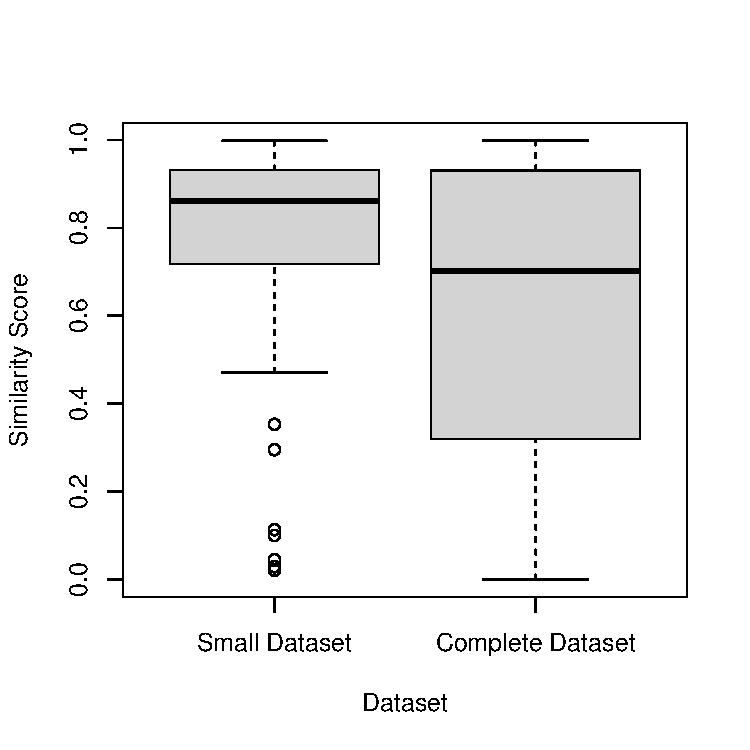
\includegraphics[width=\columnwidth]{images/similarity-1.pdf}
  \caption{\sscore of the malware samples in the small and complete datasets.}
  \label{fig:ss}
\end{figure}

Here we hypothesize that \sscore could explain
the differences of \mas we observed
when comparing the accuracy results for both
datasets. We first use Logistic Regression to test this hypothesis,
assessing the strength of the association between label correctness and
the \sscore. The logistic regression results reveal
a negative and real association ($p$-value $<$ 0.0005). This find suggests
that the \mas is more likely to assign a correct label to
a repackaged app in the cases where its \sscore with the original
app is small. This is a an unexpected result, since
we found a higher accuracy on the \sds even though
it presents a higher \sscore on average, in comparison with the \cds. 

In a further analysis, we use the \emph{K-Means} algorithm to split the
\cds into five clusters, according to the \sscore. We then
estimate the accuracy for each cluster, as
we show in Table~\ref{tab:ss-clusters}. Note that the \mas
achieves a percentage of hits close to 70\% in the clusters 1~--~4, that present an average \sscore of at most 0.76.


\tb{4}{There is a negative and real association between
  the \sscore and the \mas performance. Nonetheless,
  the \sscore does not explain the lower
accuracy of the \mas in the \cds.}

\begin{table}[ht]
  \caption{Characteristics of the clusters. Note that the percentage of
    hits decreases in the cluster with the higher average \sscore.}
 \centering
 \begin{tabular}{rrrrr}   \toprule
   cId & Total of Samples & Total of Hits & (\%) of Hits & \sscore \\ \midrule
   1 & 196 & 134 & 68.37 & 0.07 \\ 
   2 & 146 & 101 & 69.18 & 0.29 \\ 
   3 & 182 & 131 & 71.98 & 0.54 \\ 
   4 & 247 & 175 & 70.85 & 0.76 \\ 
   5 & 431 & 202 & 46.87 & 0.94 \\ \bottomrule
 \end{tabular}
 \label{tab:ss-clusters}
 \end{table}


\subsection{Assessment Based on Malware Family}

The similarity assessment we discussed in the previous
section does not explain the low performance of the
\mas on the \cds. Recall that the \cds is more heterogeneous
both in terms of similarity and malware families. So,
we hypothesize that the families of the malwares in the \cds could
better explain the poor performance of the \mas on the \cds.
Indeed, in the \cds, we identified a total of
57 families of malwares, though the most frequent
ones are \gps (198 samples),
\emph{kuguo} (44 samples), \emph{revmob} (36 samples),
and \emph{dowgin} (33 samples). Together, they
account for 67.75\% of the repackaged apps in our
complete dataset labeled as malware according to \vt.

This family distribution in the \cds is
significantly different from the family
distribution in the \sds---where the
families \emph{kuguo} (34 samples), \emph{dowgin} (12 samples),
and \emph{youmi} (5 samples) account for
73.91\% of the families considering the 69
repackaged apps \vt labels as malware in the \sds.
Most important, in the \sds, there is just one
\gps sample. This observation
leads us to a question: \emph{how does the \mas
perform when considering only the gappusin samples?}


Table~\ref{tab:gappusin} shows
the results of an accuracy assessment considering
only those particular samples in the \cds. Note that for 171 samples (86.36\%), neither the vanilla
\mas nor the \mas with traces were able to correctly identify
a repackaged version of an app as a malware. Merging the
outcomes of both approaches (that is, the vanilla \mas and
the \mas with traces), leads to a recall of
$\frac{27}{198} = 0.13$. Further, if we remove the \gps
samples from the \cds, the recall
of the \mas (vanilla + traces) increases to 0.71 (similar
to the performance of the original studies). 

\begin{table}[ht]
  \caption{Accuracy of the \mas when considering only the
  samples from the \gps family in the \cds.}
\centering
\begin{tabular}{lllr}
 \hline
 Malware & Vanilla \mas & \mas + Traces & Total \\
 \hline
 True & False & False & 171 \\ 
 True & False & True &  13 \\ 
 True & True & False &  12 \\ 
 True & True & True &   2 \\ 
 \hline
\end{tabular}
\label{tab:gappusin}
\end{table}


\tb{5}{The \mas fails to correctly
  identify 86.36\% of the samples from the \gps family
  as a malware. This is the main reason for the low
  recall of the \mas in the \cds.}

We further analyse the sample of \gps malware in our dataset, given its
relevance to the negative result we present in our paper. First,
Figure~\ref{fig:hist-gappusin} shows a histogram of the \sscore for the samples
in the \gps family. Note that mostly of the repackaged versions from the
\gps family are quite similar to the original versions (average \sscore
of 0.90, median \sscore of 0.95, and sd of 0.14). We also reengineer
a sample of 20 \gps malware (almost 10\% of the samples in this
family), using the \texttt{SimiDroid}\footnote{https://github.com/lilicoding/SimiDroid},
\texttt{apktool}~\footnote{https://ibotpeaches.github.io/Apktool/},
and \texttt{smali2java}~\footnote{https://github.com/AlexeySoshin/smali2java} tools.
Considering this sample of 20 \gps malware, the median \sscore is 0.98. In addition,
the repackaged version of the apps changes 2.73 methods, includes one new method,
and delete six methods from the original app (on median). Table~\ref{tab:simidroid-outputs} summarizes
the outputs of \texttt{SimiDroid} for this sample of \gps apps. The similarity assessment
of this sample of 20 \gps malware reveal a few modification patterns when comparing the original and the
repackaged versions of the apps. First, no sample in this random selected \gps dataset
modifies the Android Manifest file---that is, they do not require new permissions, for instance.
Moreover, 19 out of the 20 samples in this dataset  {\bf completely modifies} the
method \texttt{void onReceive(Context, Intent)}
of the class \texttt{com.games.AdReciver}. Although the results of the
decompilation process are hard to understand (due to code obfuscation),
the goal of this modification is to update the content of a \texttt{data.apk}
resource. There is no extra call to sensitive API (which hinders the
\mas to classify an asset as a malware). Figure~\ref{code:onReceive} shows
the code pattern of the \texttt{onReceive} method present in the samples. This particular modification
typically use a new method (\texttt{public void a(Context)}
the repackaged versions often introduce into the same class (\texttt{AdReciver}).

%\begin{wrapfigure}{l}{0.4\textwidth}
\begin{figure}
\begin{center}
    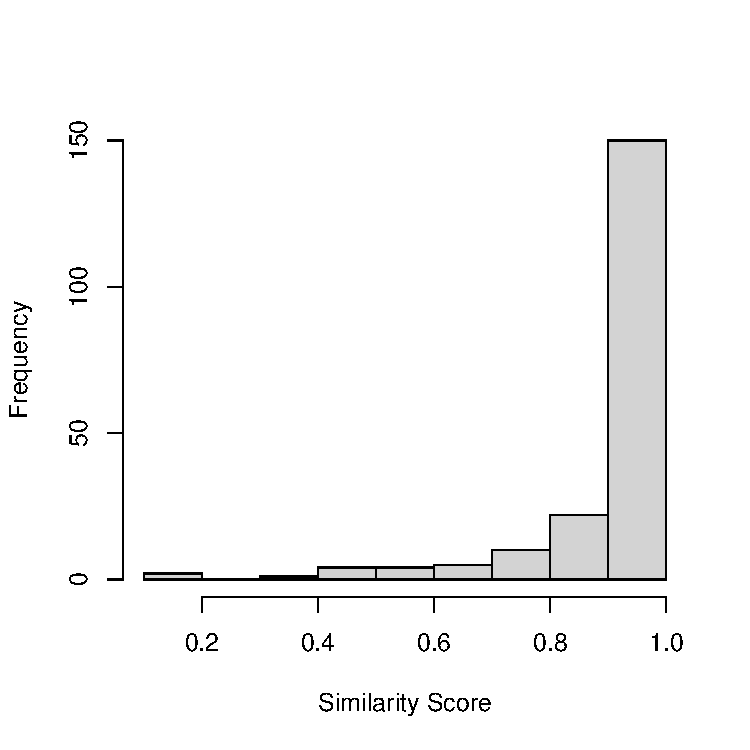
\includegraphics[width=0.38\textwidth]{images/gappusin-1.pdf}
  \end{center}
  \caption{Histogram of the \sscore for the samples in the \gps family.}
  \label{fig:hist-gappusin}
\end{figure}  
%\end{wrapfigure}

\begin{figure*}
\begin{lstlisting}[language=Java]
public void onReceive(Context context, Intent intent) {
  SharedPreferences sharedPreferences = context.getSharedPreferences(String.valueOf("com.") + "game." + "param", 0);
  int i = sharedPreferences.getInt("sn", 0) + 1;
  System.out.println("sn: " + i);
  if (i < 2) {
    mo4a(context);
    SharedPreferences.Editor edit = sharedPreferences.edit();
    edit.putInt("sn", i);
    edit.commit();
  } else if (!new C0004b(context).f7h.equals("")) {
    String str1 = context.getApplicationInfo().dataDir;
    String str2 = String.valueOf(str) + "/fi" + "les/d" + "ata.a" + "pk";
    String str3 = String.valueOf(str) + "/files";
    String str4 = String.valueOf("com.") + "ccx." + "xm." + "SDKS" + "tart";
    String str5 = String.valueOf("InitS") + "tart";
    String str6 = "ff048a5de4cc5eabec4a209293513b6e";    
    C0003a.m3a(context, str2, str3, str4, str5, str6);
    SharedPreferences.Editor edit2 = sharedPreferences.edit();
    edit2.putInt("sn", 0);
    edit2.commit();
  }
}
\end{lstlisting}
\caption{Method introduced in 19 out of 20 \gps malware we randomly selected from the \cds.}
\label{code:onReceive}
\end{figure*}

Our assessment also reveals recurrent modification patterns that {\bf delete} methods in the
repackaged version of the apps. For instance, ten repackaged apps in our
\gps sample of 20 malware remove methods from the
class \texttt{com.game.a}. These methods extensively use 
the Android reflection API, and we believe that removing these methods is
a strategy for antivirus evasion. For instance, although
specific usages of the class \texttt{DexClassLoader} might be legitimate, it allows specific
types of atack based on dynamic code injection~\cite{falsina:acsac}. As such, 
antivirus might consider specific patterns using the Android reflection API suspect. 
Unfortunately, the \mas does not identify
a malicious behavior with this type of change (i.e., changes that remove methods).
Listing~\ref{code:deletedMethod} shows an example of code pattern frequently removed
from the repackaged versions from the \gps family. 

\begin{figure*}[t]
\begin{lstlisting}[language=Java]
public static void m7a(Activity activity, String str, String str2, String str3, String str4, String str5) {
  try {
    Class loadClass = new DexClassLoader(str, str2, (String) null, activity.getClassLoader()).loadClass(str3);
    Object newInstance = loadClass.getConstructor(new Class[0]).newInstance(new Object[0]);
    Method method = loadClass.getMethod(str4, new Class[]{Activity.class, String.class});
    method.setAccessible(true);
    method.invoke(newInstance, new Object[]{activity, str5});
  } catch (Exception e) {
    e.printStackTrace();
  }
}  
\end{lstlisting}
\caption{Example of method that is typically removed from the repackaged apps of the \gps family.}
\label{code:deletedMethod}
\end{figure*}

 
\begin{table}[ht]
  \centering
  \caption{Summary of the outputs of the \texttt{SimiDroid} tool for the sample of 20
    \gps malware. (IM) Identical Methods, (SM) Similar Methods, (NM) New Methods, and
    (DM) Deleted Methods.}
  \begin{tabular}{lrrrrr}
   \toprule
    Hash & SimiScore & IM & SM & NM & DM \\ 
   \midrule
   \texttt{2D76DE7} & 0.99 & 461 &    1 &   1 &   6 \\ 
   \texttt{46C41BE} & 0.99 & 1164 &   1 &   1 &   6 \\ 
   \texttt{0218D0E} & 0.99 & 1082 &   1 &   1 &   6 \\ 
   \texttt{07EA86C} & 0.99 & 2127 &   1 &   1 &   6 \\ 
   \texttt{078E0AE} & 0.95 & 134 &   6 &   1 &  10 \\ 
   \texttt{5374927} & 0.95 & 134 &   6 &   1 &  10 \\ 
   \texttt{17722D9} & 0.97 & 265 &   6 &   1 &  10 \\ 
   \texttt{5B0C652} & 0.99 & 2642 &   4 &  10 &   1 \\ 
   \texttt{CCD29EC} & 0.99 & 436 &   2 &   0 &   0 \\ 
   \texttt{010C070} & 0.99 & 2249 &   3 &   3 &   0 \\ 
   \texttt{723C231} & 0.98 & 228 &   2 &   1 &  10 \\ 
   \texttt{27D5D22} & 0.99 & 612 &   5 &   1 &  10 \\ 
   \texttt{92209D0} & 0.99 & 698 &   2 &   3 &   0 \\ 
   \texttt{2441293} & 0.98 & 123 &   2 &   0 &  11 \\ 
   \texttt{D83F1CE} & 0.94 & 150 &   2 &   6 &   6 \\ 
   \texttt{00405B6} & 0.99 & 864 &   2 &   1 &  10 \\ 
   \texttt{33896EB} & 0.99 & 3205 &   2 &   0 &   0 \\ 
   \texttt{1AE4E8B} & 0.99 & 3964 &   2 &   3 &   3 \\
   \texttt{114C5C8} & 0.99 & 5631 &   2 &   9 & 151 \\ 
   \bottomrule
 \end{tabular}
 \label{tab:simidroid-outputs}
\end{table}

In summary, our reverse engineering effort confirm that malware
samples from the \gps family do not (a) modify the Android Manifest
files and (b) call additional sensitive APIs---reducing the hability
of the \mas to classify a sample as a malware correctly. We argue in favor
of new research efforts to integrate the \mas approach
with other techniques that could increase their performance
on malware identification. Since the samples from the \gps
family use specific patterns to introduce malicious behavior,
static analysis approaches looking at these patterns could be
an interesting alternative. 



%% \begin{figure}
%%   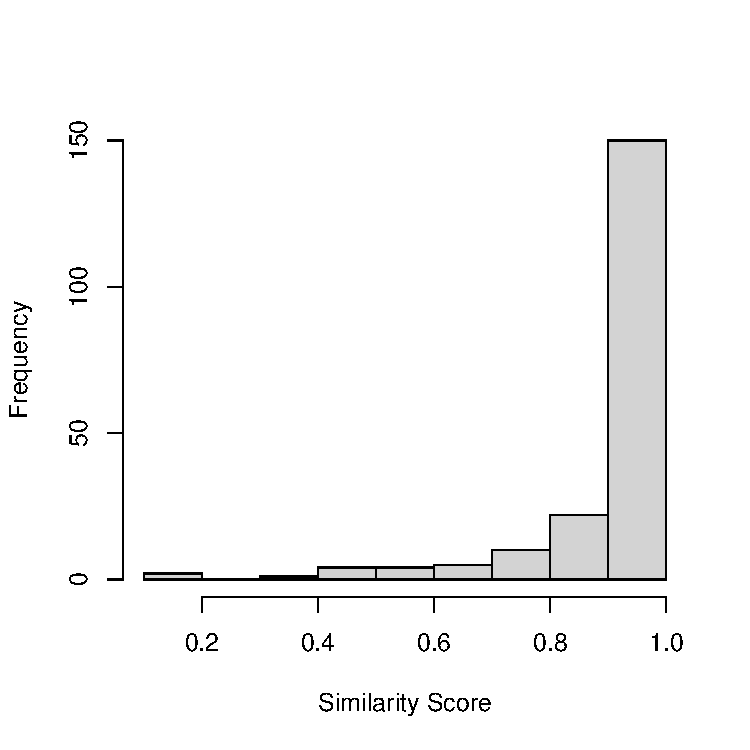
\includegraphics[scale=0.5]{images/gappusin-1.pdf}
%% \end{figure}

\todo[inline]{{\bf RB}. Removing the \gps family improves
  the recall, though did not improve precision. What is the reason
  for the low precision of \mas in the \cds? We should investigate
this issue.}


%% Considering
%% manifest analysis, as we explained in Section~\ref{sec:manifestAnalysis},
%% looking at the occurrence of duplicated permissions and duplicated 
%% components allows us to correctly classify \num{120} out of the \num{607} missed cases
%% from the mining sandbox approach (\num{19.76}\%).                                   
%% Table~\ref{tab:mfa-complete} summarizes the results of this investigation. When considering the 
%% complete dataset (\num{800} apps), combining the vanilla
%% mining sandbox approach (VMS) with trace analysis (TA) and
%% manifest analysis (MA) leads to the correct classification
%% of \num{446} malware (\num{55.75}\%), which suggests that
%% the mining sandbox approach requires further improvements when
%% we take into account a more representative dataset
%% of malware. 


%% \begin{table}[ht]
%%   \centering
%%   \begin{small}
%%   \begin{tabular}{lcc}\toprule
%%   Technique      & Hits & Recall \\ \midrule 
%%   VMS            & 193  & \num{24.12}\% \\ 
%%   VMS + TA       & 369  & \num{46.12}\%  \\
%%   VMS + MA       & 313  & \num{39.12}\% \\
%%   VMS + TA + MA  & 446  & \num{55.75}\% \\  \bottomrule
%%   \end{tabular}
%%   \end{small}
%%     \caption{Summary of the results in the Complete Dataset.}

%%  \label{tab:mfa-complete}
%% \end{table}

%% \begin{obs}{5}{}
%%   The results so far bring evidence that
%%   further research is necessary to understand
%%   the limitations of the mining sandbox approach
%%   targeting more comprehensive datasets.
%% \end{obs}

%% Our exploration of all sensitive APIs called by all app pairs brought to the light the most frequently abused sensitive APIs that
%% appear in the repackaged, malicious version of the apps. We observed that when executed all 800 app pairs, DroidBot called $75$ sensitive APIs at least one time (from our list of 162 sensitive APIs). Among them, $16$ APIs account for more than half of all calls ($51.06$\%).
%% %\rb{I could not understand the previous sentence}.
%% The sensitive API that is abused the most by repackaged apps is \textbf{android.telephony.TelephonyManager: java.lang.String getDeviceId()}, which gets the device
%% IMEI\footnote{From Wikipedia: International Mobile Equipment Identity (IMEI) is a number, usually unique, to identify 3GPP and iDEN mobile phones.}.
%% Table~\ref{tab:APIused} presents the list of the most frequent sensitive APIs that only the malicious
%% version of the apps in our dataset call.

%% \begin{obs}{6}{}
%%   The results so far bring evidence that only a handful of resources accesses like the \textbf{device id} are most attractive to malware designers, providing a potentially high-impact point of focus for future researchers and practitioners.
%% \end{obs}

%% %\begin{landscape}
%% \begin{table*}[t]
%%  \scriptsize
%%   \caption{Sensitive APIs more used by repackage apps}
%%   \centering
%%   %\begin{small}
%%  \begin{tabular}{lc}

%%    \toprule
%%    Sensitive API & Occurrences \\
%%    \midrule
%%    01 android.telephony.TelephonyManager: java.lang.String getDeviceId() &  78 \\
%%    02 android.net.wifi.WifiManager: android.net.wifi.WifiInfo getConnectionInfo() &  64\\
%%    03 android.net.wifi.WifiInfo: java.lang.String getMacAddress() &  63 \\
%%    04 android.net.NetworkInfo: java.lang.String getTypeName() &  58 \\
%%    05 android.net.NetworkInfo: java.lang.String getExtraInfo() &  56 \\
%%    06 android.telephony.TelephonyManager: java.lang.String getSubscriberId() &  54 \\
%%    07 android.net.NetworkInfo: android.net.NetworkInfo State getState() &  52 \\
%%    08 android.database.sqlite.SQLiteOpenHelper: android.database.sqlite.SQLiteDatabase getWritableDatabase() &  49 \\
%%    09 android.database.sqlite.SQLiteDatabase: android.database.Cursor query(java.lang.String, ...,java.lang.String) &  47 \\
%%    10 android.telephony.TelephonyManager: java.lang.String getNetworkOperator() &  45\\
%%    11 android.telephony.TelephonyManager: android.telephony.CellLocation getCellLocation() &  44\\
%%    12 android.database.sqlite.SQLiteOpenHelper: android.database.sqlite.SQLiteDatabase getReadableDatabase() &  44\\
%%    13 android.telephony.gsm.GsmCellLocation: int getLac() &  42 \\
%%    14 android.telephony.gsm.GsmCellLocation: int getCid() &  42 \\
   
%%    15 android.net.ConnectivityManager: android.net.NetworkInfo getNetworkInfo(int) &  39 \\
%%    16 android.telephony.TelephonyManager: java.lang.String getNetworkOperatorName() &  36 \\
%%    .&  .\\
%%    .&  .\\
%%    .&  .\\
%%    74 android.app.ActivityManager: java.util.List getRecentTasks(int,int) & 1 \\
%%    75 android.net.NetworkInfo: java.lang.String toString() & 1 \\

%%  \bottomrule
%%                             Total & 1592 \\

%%  \end{tabular}
%%  %\end{small}
%%  \label{tab:APIused}
%% \end{table*}
%\end{landscape}

%% \begin{obs}{1}{}
%%    %\kn{Here we need to add some final take aways of the reproduction study}
%%    Our results indicate that in the presence of a representative dataset ($800$ app pairs as opposed to $102$ and a diverse similarity index), the accuracy of state of the art in mining sandbox approaches, using DroidBot drops significantly (from $63.36\%$ to $24.12\%$). Our results also indicate that only few sensitive APIs are responsible for majority of injected malware in repackaged apps. This encourages the emergence of new proposals that can support mine sandbox mitigating \textit{blindspot}s that lead to low accuracy.
%%  \end{obs}


%\kn{In this subsection, are we simply reproducing the results of existing papers. Because as far as I understand, tools like DroidBOT etc. were evaluated by simply comparing the sensitive APIs call. I am guessing here our contribution is to evaluate it on the larger dataset. I have given it a shot, please keep me posted if this is correct.}

%% \subsection{Trace Analysis Results}\label{sec:traceResults}

%% In this section, we describe the results of our investigation on how the trace from the entry point to sensitive API could impact the accuracy of sandbox approaches. Initially, we collect the call graphs of DroidBot execution using \emph{Logcat} and filter in the traces between the app's entry point and calls to any sensitive methods.

%% Then, using the callgraph from executions of both app versions (benign/malicious), we track the differences between their traces. We choose to investigate only app pairs that covered the same set of sensitive APIs detected in both versions during our first experiment (Section~\ref{sec:Sensitive APIs}). 


%% \begin{obs}{2}{}
%%  The state of the art in mining sandbox approaches using DroidBot have a blind-spot when it comes to being aware of the trace taken from the entry point to a sensitive API call. The approaches could have a improvement of $22\%$ if it considered trace as a factor. Similar  improvements are also seen with the original dataset of $101$ app pairs (improvement of $18.81\%$).
%%  \end{obs}

%% \subsection{Manifest File Analysis}\label{sec:manifestResults}

%% In this section, we describe the results of our investigation on the impact of modified manifest files on the accuracy of sandbox approaches. 
%% To this end, we check some particulars from manifest file, that point to a likely suspicious behavior. In section \ref{sec:manifestAnalysis}, we illustrated that an automatic hacking script could inject permission requests at manifest file regardless of whether this request is already present on it, which can result in duplicated permission and actions in the Manifest file. We looked out for such modifications in the malware that went undetected by the test generation tools. Table~\ref{tab:mfa} summarizes our results.


%% The column (SAPI) indicates the number of malware that went undetected during our first study (same as Table~\ref{tab:pa}'s Same API set (SAPI)). The second column (DP) indicates how many Manifest files from malicious app undetected at first study, had duplicated permission. Same way, column (DA) denotes the number of Manifest files with the duplicated actions in their manifest file.

%% A duplicate request for permission or action in a malicious version's manifest file should have been performed by a script. A simple analysis of manifest file could detect $120$ of undetectable malware from the first experiment ($607$), if it considers explorer duplicate permissions or actions at manifest file code as a detection strategy. If we combine the previous trace analysis with manifest file analysis, we improve the accuracy rate to $55.75\%$.

%% It is to be noted that in the presence of the original dataset of $101$ app pairs, the manifest file analysis combined with the trace analysis earlier discussed improves the accuracy rate to $90.09\%$ confirming that such an analysis, even though naive and simple does have an impact on the accuracy rate of mining sandbox approaches.  %\kn{Handrick as before please put the full numbers in the table}


%% \begin{obs}{3}{}
%%  We can conclude that sandbox approach also could have better accuracy if they considered the suspicious modifications in manifest file in their analysis. Although the analysis required of the manifest file is quite naive, we believe the results present an interesting and relevant insight for developers of malware detection tools to improve accuracy.
%% \end{obs}

%% \todo[inline]{rb: I reviewed the paper until this point. I think that next we should
%% provide more explicit answers to the research questions. kn: Given this a shot}

%% \todo[inline]{mm: any finding we want to formulate related to the discussion in the last paragraph? kn: Given it a shot}

